\chapter{Evaluation}	
The evaluation is divided into two sections, one for each development method used. In each section, the developed application, it's structure and functionality is presented, followed by the results of the code evaluation. 

\section{Native android} \label{android}
The developed native application can be cloned from Github at [..], also a compressed version of all source code used in the thesis can be found at [..]. An overview of the application structure and functionality follows in section ~\ref{sec:nativestructure}. 

\subsection{Application structure} \label{sec:nativestructure}
A UML-diagram representing the Android application can be seen in figure ~\ref{fig:nativeuml}, with the classes summarized below.

\begin{description}
	\item[MainActivity] is the main activity of the program. It is in charge of starting activities upon request from the web application, and registers 
	
	
	\item[IntentFactory] provides intents for native functions such as capturing an image or picking an image from the gallery.
	\emph{Ex. getting intent from intent factory}\\
	
	\begin{lstlisting}
		// In Bridge:
		Intent imageIntent = IntentFactory.createCameraIntent(context);
		
		// In IntentFactory:
public static Intent createCameraIntent(Context context) {
        // Create the intent for capturing an image
        Intent takePictureIntent = new Intent(MediaStore.ACTION_IMAGE_CAPTURE);

        // Ensure that there's a camera activity to handle the intent
        if (takePictureIntent.resolveActivity(context.getPackageManager()) != null) {
            // Create the File where the photo should go
            File photoFile = AndroidHardware.requestImageFile();
            takePictureIntent.putExtra(MediaStore.EXTRA_OUTPUT,
                    Uri.fromFile(photoFile));
        }
        return takePictureIntent;
    }
	\end{lstlisting}
	
	\item[AndroidHardware] handles hardware related logic, such as file creation.
	
	\item[Bridge] serves as a bridge between the native application and web. When a native function is requested, Bridge requests the corresponding Intent from IntentFactory, and creates a Callback of the corresponding type. The Intent is sent to MainActivity for execution, and the Callback is stored in MainActivity.
	
	\item[WebViewDataSender] is the class communicating back to the web application by invoking javascript-functions in the browser.
	
	\item[JsInterface] is exposed to the web application as a JavaScriptInterface and acts as a receiver for function calls from the web application. Whenever native functionality is needed, the javascript in the web application can call upon it's methods. JsInterface forwards the function calls to Bridge, which in turn, contains the logic for each function.
	
	\item[Callback] contains logic specifying how to send results from a native function back to the web application.
	
	\begin{description}
		\item[ImageCallback] is used when the web application requests an image from the camera.
		
		\item[ImagePickCallback] is used when the web application requests an image from the gallery.
		
	\end{description}
	\item[UniqueInteger] is used by MainActivity when storing callbacks. An unique integer is used as an id for an Intent and its related callback. Upon completion of an Intent, the Callback with the same id is executed.
	
\end{description}

\begin{figure}[h!]
	\centering
    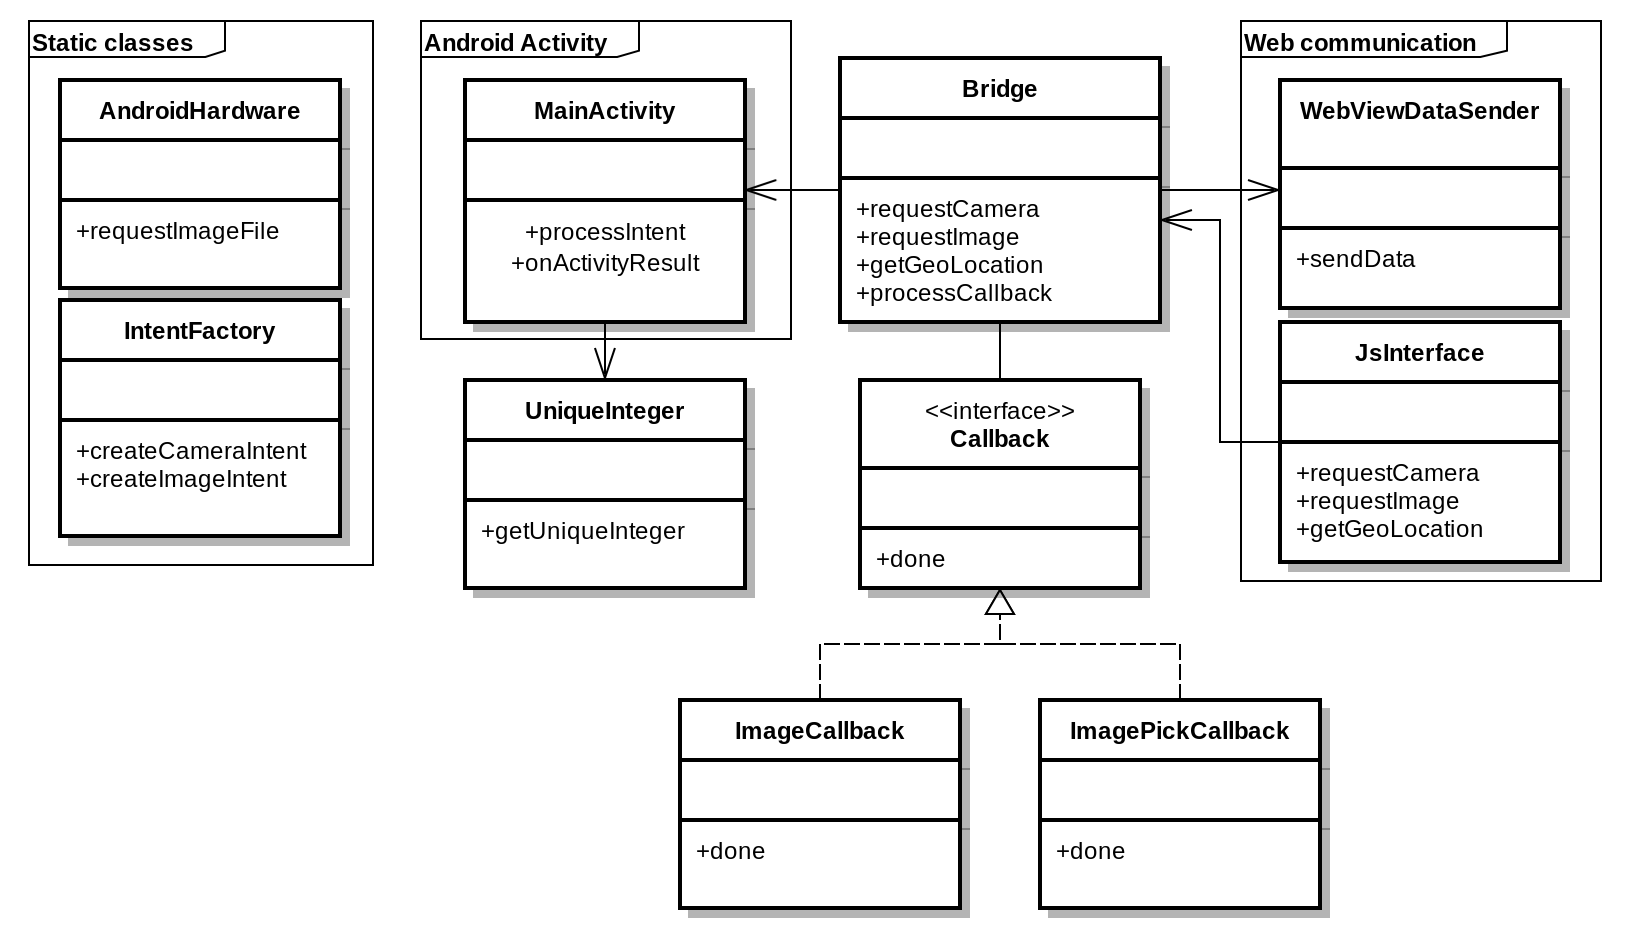
\includegraphics[width=120mm,natwidth=800,natheight=600]{./img/polluxuml.png}
    \caption{Structure of the android application}
    \label{fig:nativeuml}
\end{figure}

In order to simplify development of the web application with support for both web browsers and the Android application, part of the logic follows the adapter pattern. The business logic of the web application stays the same, and only the communication with the unit (web browser or application), for example when uploading a picture, differs. Figure ~\ref{fig:nativewebuml} displays the basic structure of the web application. 

\begin{figure}[h!]
	\centering
    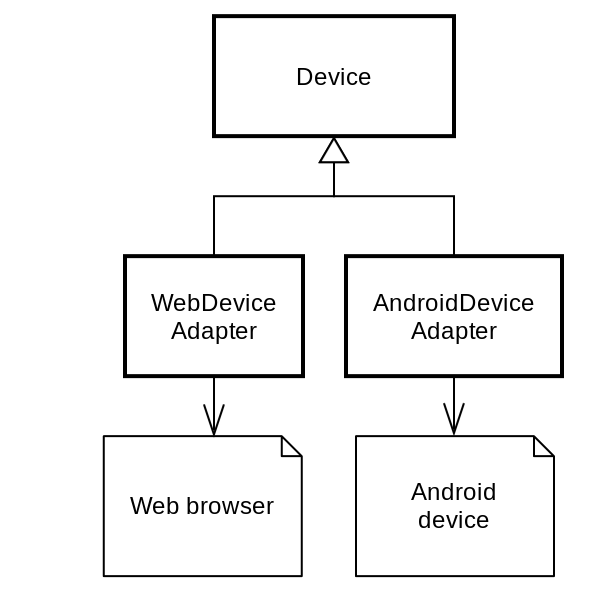
\includegraphics[width=60mm,natwidth=400,natheight=300]{./img/androidwebuml.png}
    \caption{Structure of the web application}
	\label{fig:nativewebuml}
\end{figure}

A more detailed view of the program flow when the web application requests an image can be seen in figure ~\ref{fig:nativeflow}, further explained below.
\begin{figure}[h!]
	\centering
    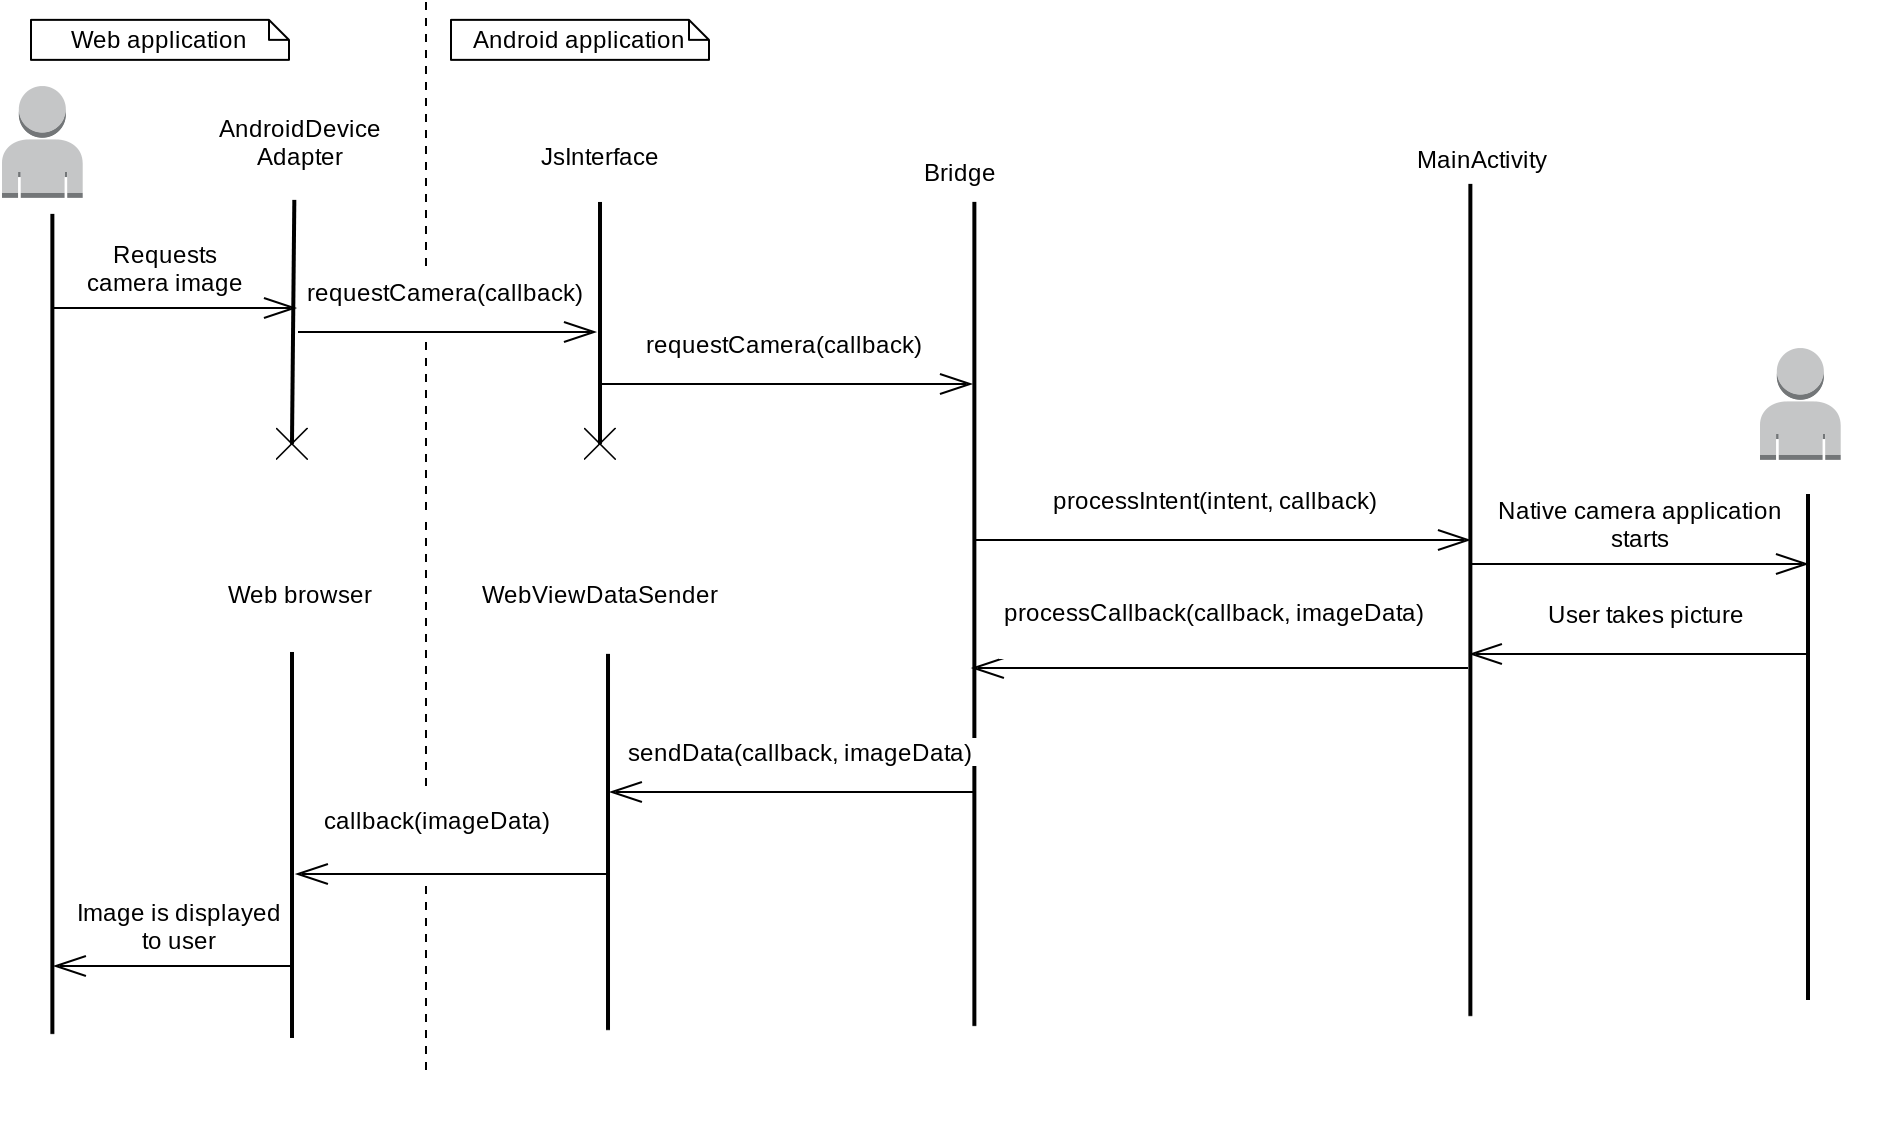
\includegraphics[width=120mm,natwidth=800,natheight=600]{./img/androidfunctionflow.png}
    \caption{Function flowchart, single call from web application}
    \label{fig:nativeflow}
\end{figure}
\begin{enumerate}
	\item User action invokes a request for an image from the mobile camera
	\item Current device adapter (AndroidDeviceAdapter) calls requestCamera on JsInterface, with the function name of the preferred callback function as argument
	\item JsInterface forwards the function call to Bridge
	\item Bridge creates the corresponding Intent and Callback, and calls processIntent on MainActivity with Intent and Callback as arguments
	\item MainActivity Creates gets a unique id from UniqueInteger, stores the callback in a hashmap with the id as key, and starts the intent with the id as requestcode.
	\item Camera application starts
	\item When user takes a picture, MainActivity gets notified by the Android system, pulls the Callback with the same id as the processed Intent, and forwards the callback and resulting image data to Bridge through processCallback
	\item Bridge executes the callback which in turn calls sendData on WebViewDataSender, with the image data and callback name as arguments
	\item WebViewDataSender executes the javascript callback function in the browser window
	\item The captured image is displayed to the user in the browser
\end{enumerate}

\subsection{Code evaluation}
Evaluation of the developed application was performed as described in [...], and a summary of the results  can be seen in the table below.

\begin{tabular}{ | l | c | r | }
    \hline
    \multicolumn{3}{|c|}{Quantitative metrics} \\
    \hline
	Metric & Android application &  Web application \\
	\hline
	Files & 10 & 2\\
	LLoC & 200 & 173\\	
	\hline
	\multicolumn{3}{c}{\emph{Result of code evaluation using ProjectCodeMeter}}
\end{tabular}

\section{PhoneGap}
The developed PhoneGap application can be cloned from Github at [..], also a compressed version of all source code used in the thesis can be found at [..]. An overview of the application structure and functionality follows in section ~\ref{sec:phonegapstructure}. 

\subsection{Application structure} \label{sec:phonegapstructure}
A UML-diagram representing the PhoneGap application can be seen in figure ~\ref{fig:phonegapuml}, with the classes summarized below.
\begin{figure}[h!]
	\centering
    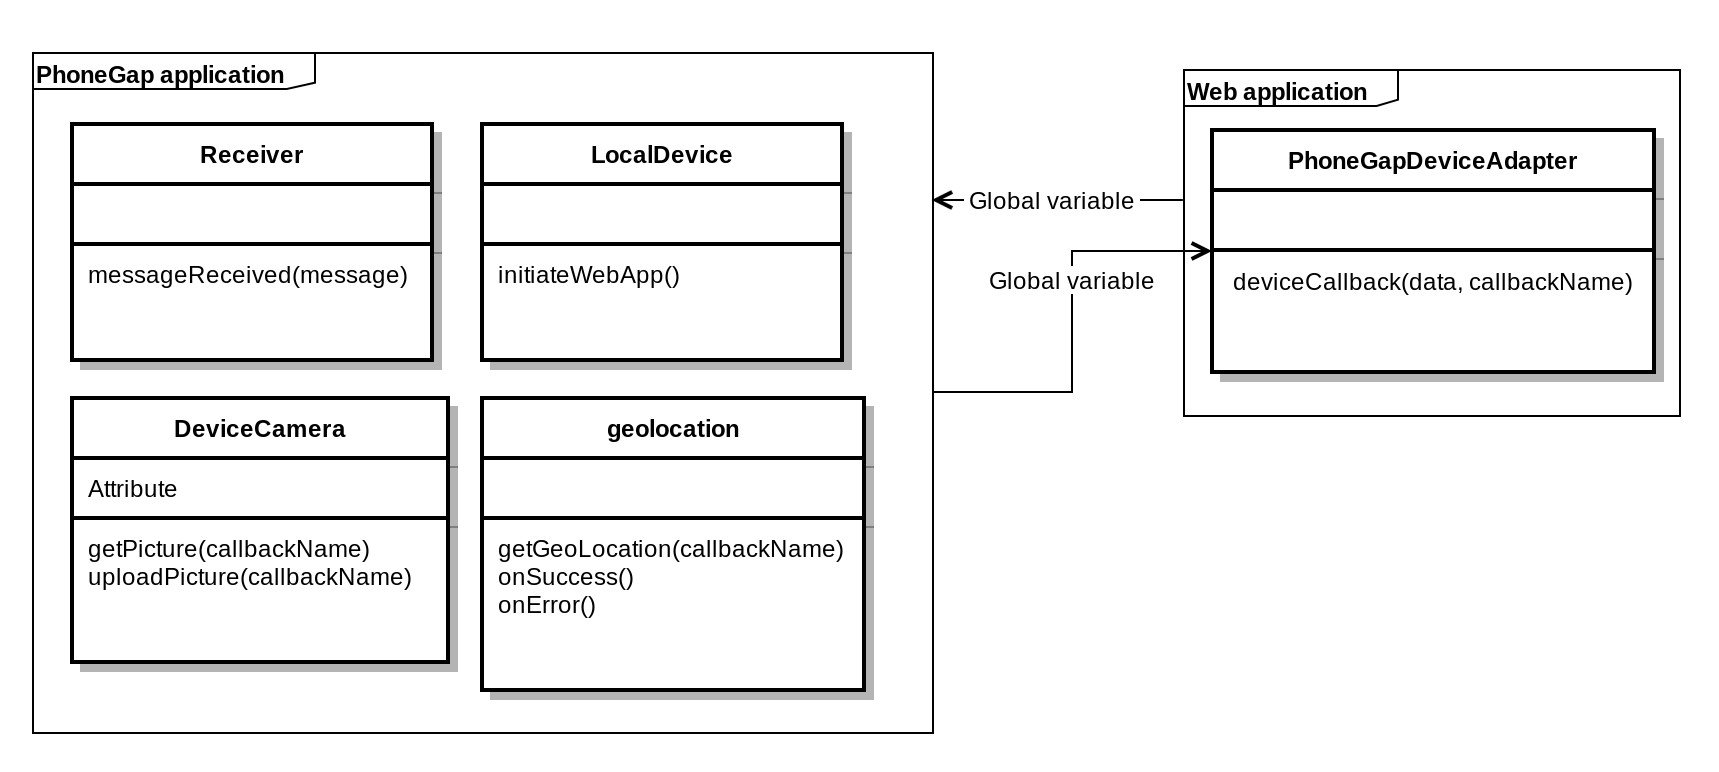
\includegraphics[width=120mm,natwidth=800,natheight=600]{./img/phonegapuml.png}
    \caption{Structure of the phonegap application}
    \label{fig:phonegapuml}
\end{figure}

\begin{description}
	\item[Receiver] listens to messages posted to the browser window PhoneGap is running in. Receives messages from web application and calls the requested methods in the PhoneGap application.
	\item[LocalDevice] is used to load the web application and initialize the device in the web application to the correct adapter.
	\item[DeviceCamera] contains logic for invoking, and receiving results from the device camera. Also forwards the results to the web application.
	\item[geolocation] contains logic for accessing the phones geo location (GPS-position) and forwarding the results to the web application.
\end{description}


In order to simplify development of the web application with support for both web browsers and the PhoneGap application, part of the logic follows the adapter pattern. The business logic of the web application stays the same, and only the communication with the unit (web browser or application), for example when uploading a picture, differs. Figure ~\ref{fig:phonegapwebuml} displays the basic structure of the web application. 

\begin{figure}[h!]
	\centering
    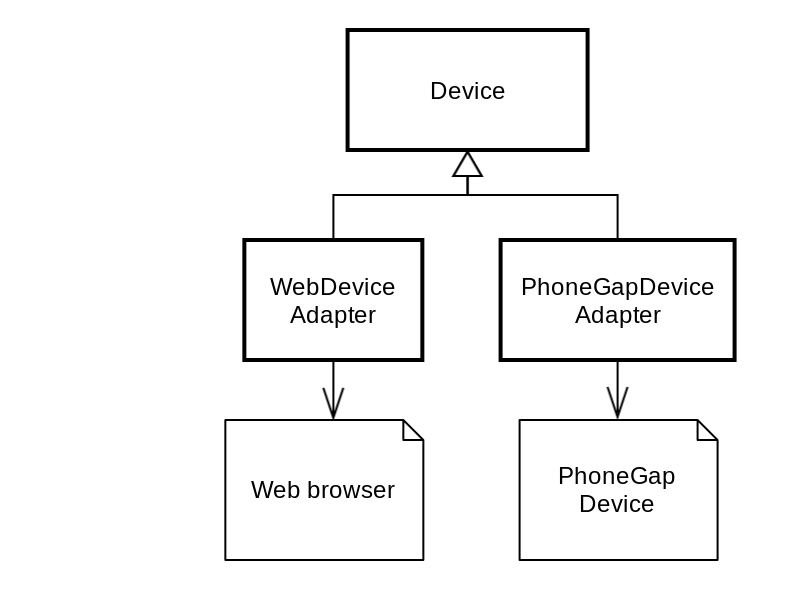
\includegraphics[width=60mm,natwidth=400,natheight=300]{./img/phonegapwebuml.png}
    \caption{Structure of the web application}
        \label{fig:phonegapwebuml}
\end{figure}

\begin{figure}[h!]
	\centering
    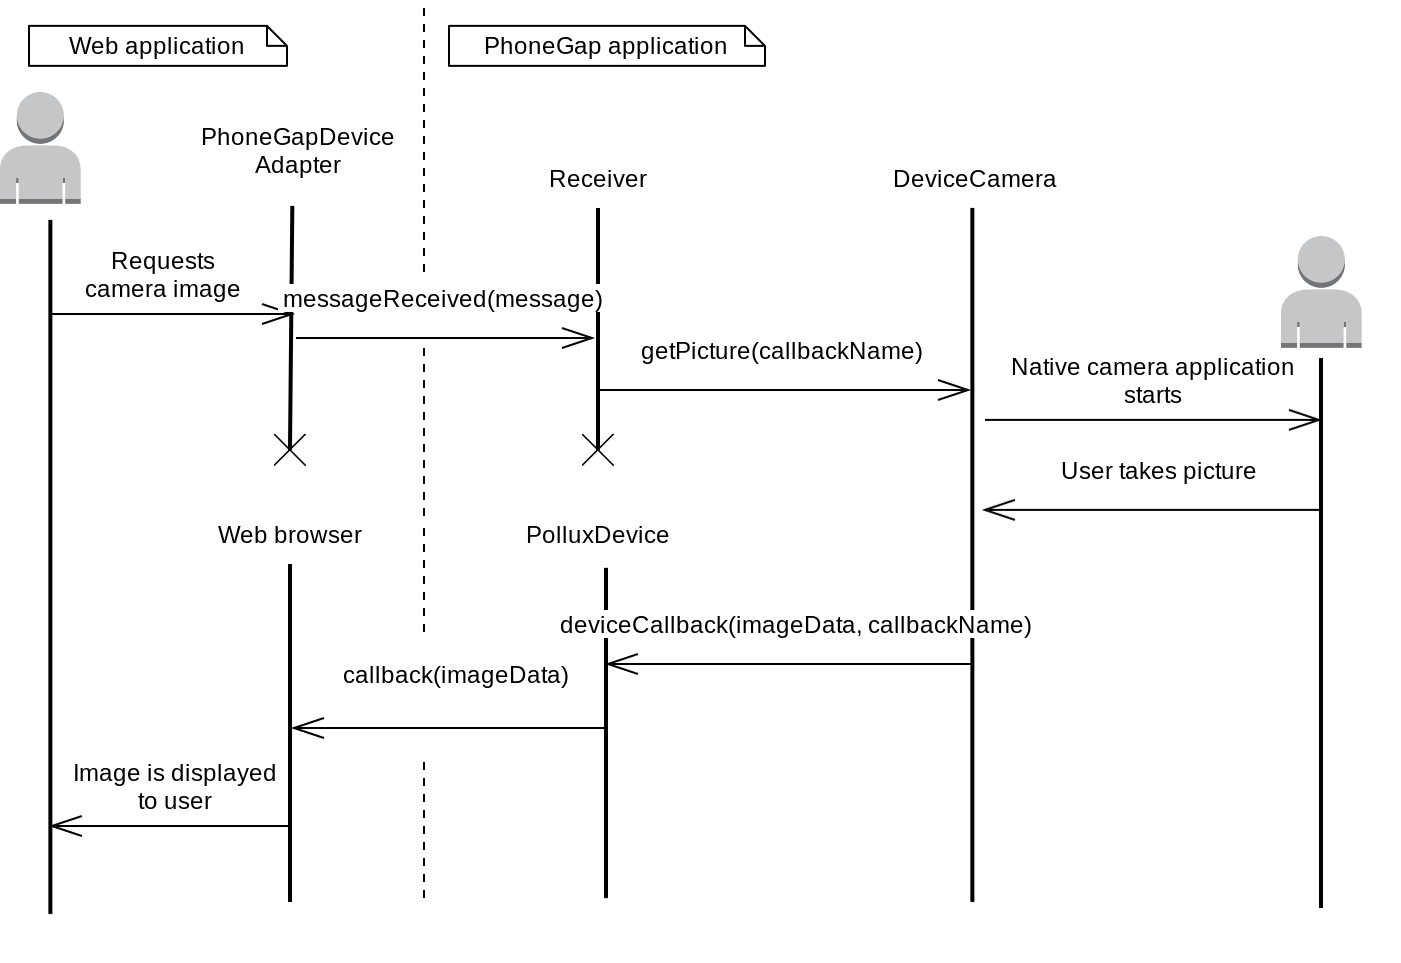
\includegraphics[width=120mm,natwidth=800,natheight=600]{./img/phonegapfunctionflow.png}
    \caption{Function flowchart, single call in web application}
\end{figure}
\begin{enumerate}
	\item User action invokes a request for an image from the mobile camera 
	\item Current device adapter (PhoneGapDeviceAdapter) forwards the request to the PhoneGap application using postMessage
	\item The message gets processed by the PhoneGap receiver which forwards the call to DeviceCamera via the getPicture function
	\item DeviceCamera uses PhoneGap library code to start the camera application
	\item User takes picture, and the result is received by DeviceCamera
	\item DeviceCamera returns the result to the browser by invoking DeviceCallback on the exposed javascript object, in PhoneGap known as PolluxDevice
	\item DeviceCallback calls the javascript callback function specified in its argument
	\item The captured image is displayed to the user in the browser	
\end{enumerate}

\subsection{Code evaluation}
Evaluation of the developed application was performed as described in [...], and a summary of the results  can be seen in the table below.

\begin{tabular}{ | l | c | r | }
    \hline
    \multicolumn{3}{|c|}{Quantitative metrics} \\
    \hline
	Metric & PhoneGap application &  Web application \\
	\hline
	Files & 3 & 2\\
	LLoC & 86 & 175\\	
	\hline
	\multicolumn{3}{c}{\emph{Result of code evaluation using ProjectCodeMeter}}
\end{tabular}